% \section{Prospects} \label{prospects}
% \subsection{Advanced Onboard Processing (REMOVE)}
% \hl{Sivert, Joe \\}
% Readily compressed and reduced data containing a few relevant spectral signatures across geo-referenced coordinates may efficiently be transmitted to ground enabling faster operational response to investigate target(s) in-situ.

% Super-resolution algorithms may be developed to enhance the spatial resolution \cite{Park2003, Garrett2019} and provide improved detectability of features of interest. The latter may give more accurate classification and target detection with fine spatial resolution and high spectral resolution in the image \cite{Manolakis2002, Manolakis2005, Bakken2019SPIE}.

% On-the-Fly-Processing (OTFP) compression and dimensionality reduction for high-dimensional data streams may  also be employed with marginal loss of useful systematic information while improving SNR \cite{Vit17}. 

% \subsection{Constellation and Multi-agent architecture (REMOVE)}
% \hl{Mariusz, Roger \\}
% \begin{figure}[!b]
% 	\begin{center}
% 	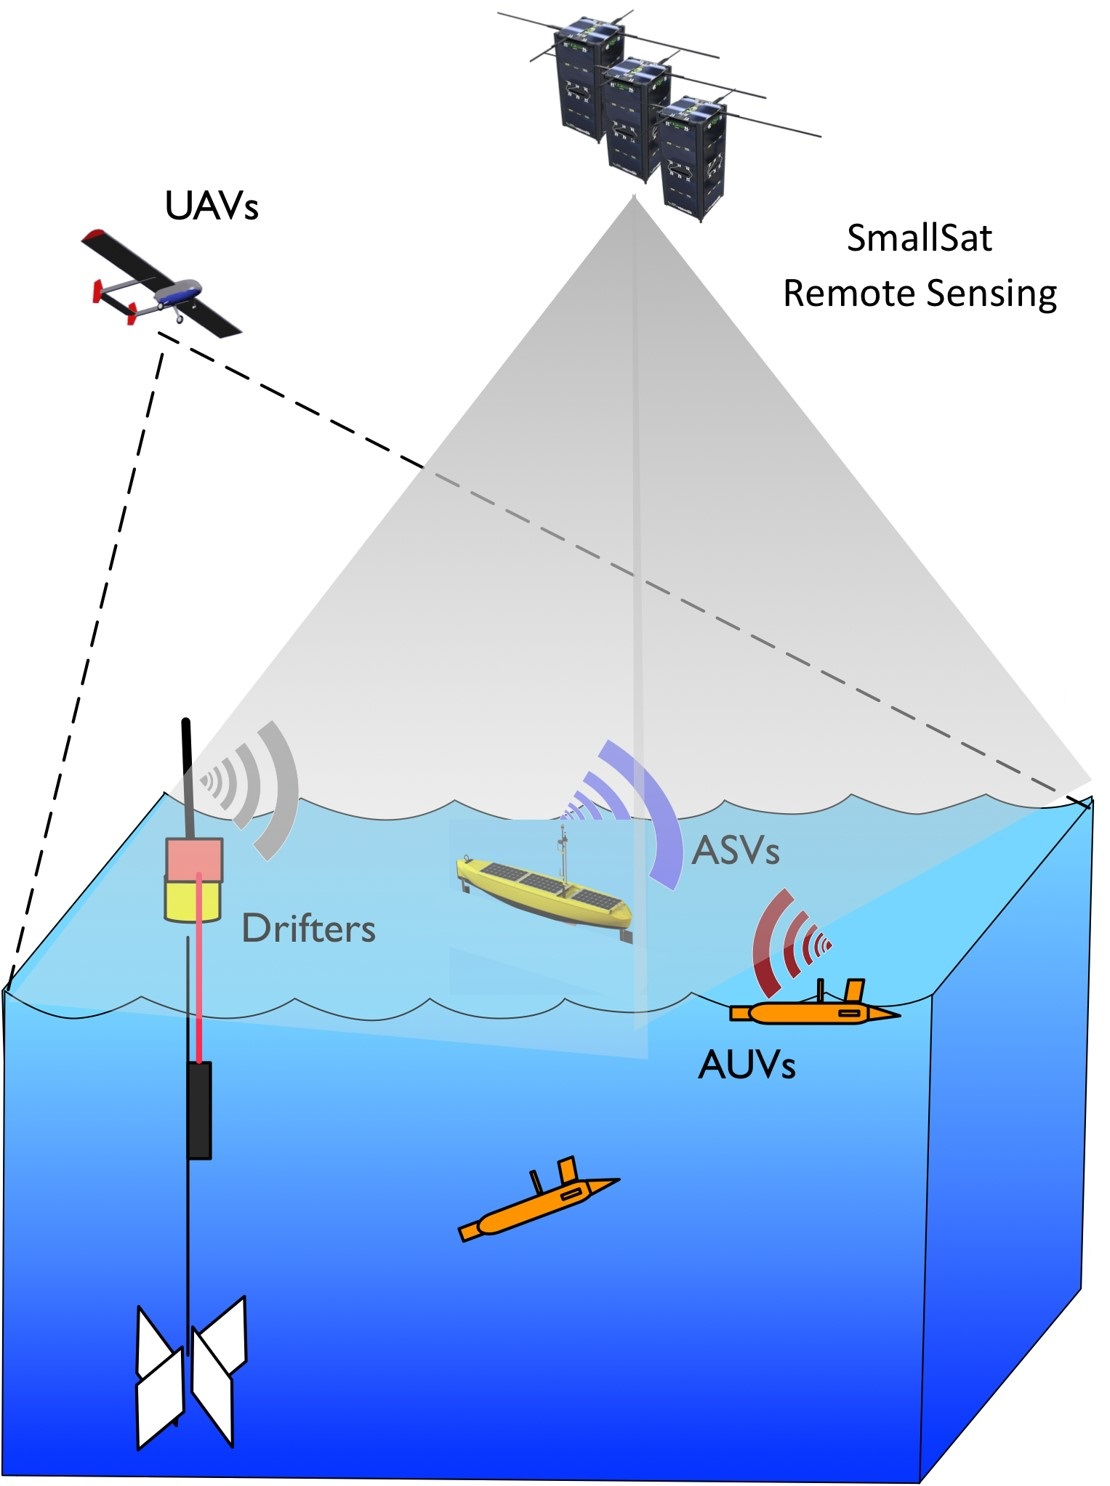
\includegraphics[width=60mm,angle=0]{figs/overview2.jpg}
% 	\caption{Illustration of the main components in a multi-agent marine observation system.}
% 	\label{fig:overview}
% 	\end{center}
% \end{figure}
% A network of autonomous underwater vehicles (AUVs), autonomous surface vehicles (ASVs) and unmanned aerial vehicles (UAVs) is capable of coordinated missions executed in concert with conventional vehicles, buoys and fixed sensor networks as envisioned in Autonomous Ocean Sampling Network (AOSN) \cite{Bel93,Far14}. Such systems enable not only significant reduction in operational costs, and increased safety, but more importantly provide substantially more and continuous information about the observed targets and features of scientific interest. These networks take advantage of the complementary and coordinated capabilities of such autonomous assets related to position, range, endurance, mobility, sensors, and across large spatio-temporal scales for \emph{synoptically} observing an oceanographic phenomenon. Figure \ref{fig:scales} illustrates the complementary capabilities of the different platforms, and shows the scope for a coordinated observation system that exploits the advantages of each platform type. 
% \begin{figure}[tbhp]
%   \begin{center}
%     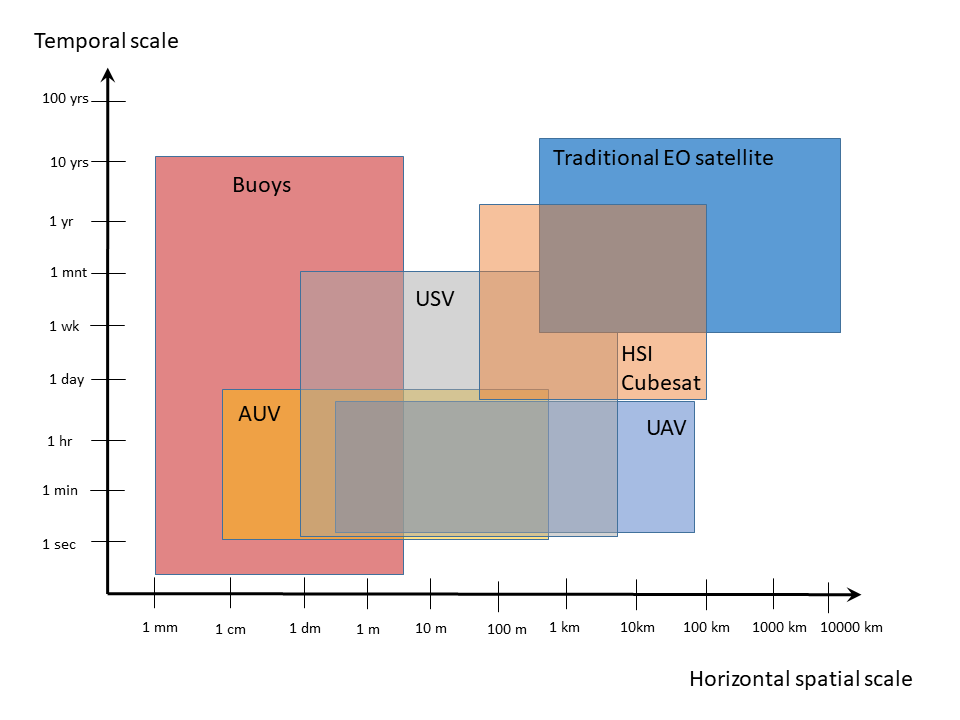
\includegraphics[width=90mm,angle=0]{figs/scales.png}
%     \caption{Mapping of capabilities of various sensor platforms used
%       for ocean color.}
%     \label{fig:scales}
% \end{center}
% \end{figure}
% It is clear that a constellation of multiple small-satellites hosting HSI small-satellites will extend the capability in all dimensions. It can also be observed that a HSI on a satellite is a useful and complementary platform to AUVs, USVs, UAVs and buoys/drifters given the limited mobility and speed of the mentioned platforms. In particular, the capabilities covered by satellites, UAV and USV are very well aligned with requirements for observing highly dynamic events such as phytoplankton blooms \cite{Dic05}. 

% Figure \ref{fig:scales} summarizes the typical capabilities of the different robotic platforms in a marine observation system. The rightmost end of the horizontal spatial capability defines the spatial coverage of the HSI, while the leftmost defines the smallest spatial scales that can be captured by a HSI on the platform. The upper end of the temporal capability defines the endurance of the platform, while the lower end illustrates the revisit time or fastest temporal scales that can be observed. Another important dimension is related to the maximum speed of UAVs, USVs and AUVs implying that high temporal and spatial resolution can only be achieved within limited parts of areas that are within their range. This means that these type of vehicles will need adaptive sampling and be guided towards parts of the target area where informative observations can be made \cite{Bel93,fossum18,fossum18b}. Other important dimensions are related to weather sensitivities, payload weight limitations, and operational complexity.

% The components of such an autonomous multi-agent \emph{cyber-physical system} must be tightly knit together by communication technology in combination with intelligent information processing and coordinated control as well as mission planning where tasks are dynamically allocated amongst the available assets and systems. Coordination in such a context would involve observing the same patch of the ocean co-temporally across diverse assets with a range of sensing techniques to piece together a comprehensive and cogent view.
